\documentclass[aspectratio=169]{beamer}

% --- Theme & Colors ---
\usetheme{Madrid}
\usecolortheme{beaver}
\setbeamercolor{structure}{fg=darkred}

% --- Packages ---
\usepackage{graphicx}
\usepackage{booktabs}
\usepackage{tikz}
\usetikzlibrary{positioning, shapes, arrows.meta, matrix, fit, backgrounds}
\usepackage{pgfplots}
\pgfplotsset{compat=1.17}

\usepackage{tabularx}  % For auto-width columns
\usepackage{ragged2e}  % For better text wrapping

% Title Information
\title[Bank Artos to Bank Jago]{Business Model Transformation of \\ Bank Artos to Bank Jago}
\subtitle{From Legacy Pipeline to Digital Ecosystem}
\author[Kelompok 1]{Jon Felix Germinian \and Jose Galbraith Hasintongan \and Muhammad Firdaus \and Samuel Mualatua Jeremy N}
\institute[MIK]{Faculty of Computer Science \\ Universitas Indonesia}
\date{\today}

\begin{document}

% --- Slide 1: Title ---
\begin{frame}
	\titlepage
\end{frame}

% --- Slide 2: Introduction ---
\begin{frame}{Introduction}
	\begin{columns}
		\column{0.6\textwidth}
		\textbf{The Context:}
		\begin{itemize}
			\item Digital transformation is essential for survival in Indonesian banking.
			\item Intense competition from FinTechs and Neobanks.
		\end{itemize}

		\vspace{0.5cm}

		\textbf{The Case Study: Bank Jago}
		\begin{itemize}
			\item \textbf{Origin:} \textit{Bank Artos} (1992), a conventional BUKU I bank.
			\item \textbf{Turning Point:} Acquired in 2019 by MEI \& Wealth Track.
			\item \textbf{Significance:} A radical shift from legacy "Pipeline" to digital "Ecosystem".
		\end{itemize}

		\column{0.4\textwidth}
		\centering
		% Timeline Visualization
		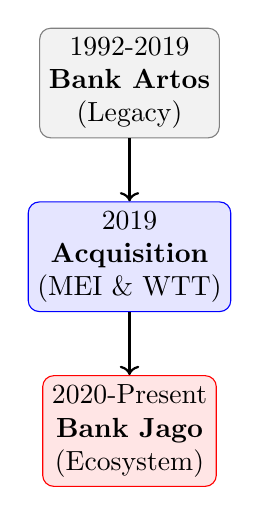
\begin{tikzpicture}[node distance=0.8cm]
			\node (artos) [rectangle, draw=gray, fill=gray!10, align=center, rounded corners] {1992-2019 \\ \textbf{Bank Artos} \\ (Legacy)};
			\node (acq) [rectangle, draw=blue, fill=blue!10, align=center, rounded corners, below=of artos] {2019 \\ \textbf{Acquisition} \\ (MEI \& WTT)};
			\node (jago) [rectangle, draw=red, fill=red!10, align=center, rounded corners, below=of acq] {2020-Present \\ \textbf{Bank Jago} \\ (Ecosystem)};
			\draw[->, thick] (artos) -- (acq);
			\draw[->, thick] (acq) -- (jago);
		\end{tikzpicture}
	\end{columns}
\end{frame}

% --- Slide 3: Theoretical Frameworks ---
\begin{frame}{Literature Review \& Frameworks}
	To analyze the transformation, two primary frameworks were employed:

	\begin{block}{1. Applegate’s Business Model Framework (2009)}
		\begin{itemize}
			\item \textbf{Strategy:} Market positioning (Product-Push $\to$ Customer-Pull).
			\item \textbf{Capabilities:} Resources, Processes, IT Infrastructure.
			\item \textbf{Value:} Economic logic and cost structures.
		\end{itemize}
	\end{block}

	\begin{block}{2. Savage’s Management Generations}
		\begin{itemize}
			\item \textbf{Gen 2/3 (Industrial/Matrix):} Rigid hierarchies and silos (Legacy Banks).
			\item \textbf{Gen 5 (Knowledge Networking):} Agile, cross-functional teaming (Digital Banks).
		\end{itemize}
	\end{block}

	\centering
	\vspace{0.2cm}

\end{frame}

% --- Slide 4: The Legacy State (Artos) ---
\begin{frame}{The Legacy State: Financial Distress (2018-2019)}
	\begin{columns}
		\column{0.5\textwidth}
		\textbf{Bank Artos Challenges:}
		\begin{itemize}
			\item \textbf{Model:} Traditional "Pipeline" (Deposit $\to$ Loan).
			\item \textbf{Reach:} Limited branches in Bandung/Jakarta.
			\item \textbf{Cost Structure:} Unsustainable.
		\end{itemize}
		\vspace{0.5cm}
		\textit{High BOPO (Operating Expenses to Operating Income) indicated the bank was bleeding cash.}

		\column{0.5\textwidth}
		\centering
		% Financial Bar Chart
		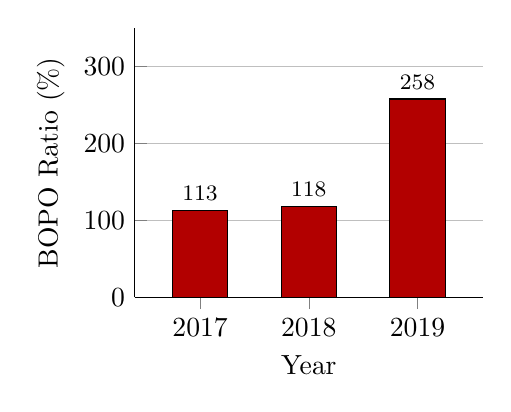
\begin{tikzpicture}
			\begin{axis}[
				ybar,
				symbolic x coords={2017, 2018, 2019},
				xtick=data,
				xlabel={Year},
				% --- FIXES START HERE ---
				ylabel={BOPO Ratio (\%)},
				ylabel near ticks,      % Fixes label overlapping numbers
				enlarge x limits=0.3,   % Adds space on left/right so bars don't hit edge
				ymin=0, ymax=350,       % Increased height so "258" isn't cut off
				nodes near coords style={font=\footnotesize}, % Makes numbers slightly smaller
				% ------------------------
				nodes near coords,
				bar width=20pt,
				width=6cm, height=5cm,
				axis lines*=left,       % Clean look (removes top/right box lines)
				ymajorgrids=true,       % Adds grid lines for readability
				]
				\addplot[fill=red!70!black] coordinates {(2017,113) (2018,118) (2019,258)};
			\end{axis}
		\end{tikzpicture}
		\vspace{0.2cm}
		\footnotesize{\textbf{BOPO > 100\% = Loss Making}}
	\end{columns}
\end{frame}

\begin{frame}{Financial Decomposition (Pre-Transformation)}
	\centering
	\renewcommand{\arraystretch}{1.5} % More breathing room for numbers
	
	% Using tabularx to fill 90% of slide width
	\begin{tabularx}{0.9\textwidth}{X c c c}
		\toprule
		\textbf{Metric} & \textbf{2017} & \textbf{2018} & \textbf{2019} \\ 
		\midrule
		Net Profit (Loss) & IDR 10.2 B & IDR 23.3 B & IDR 165 B \\ 
		BOPO & 113.70\% & 118.02\% & 258.09\% \\ 
		NPL (Net) & Low & 4.49\% & 0.05\%* \\ 
		LDR & 76.74\% & 73.42\% & 52.80\% \\ 
		NIM & 4.84\% & 4.87\% & 2.05\% \\ 
		\bottomrule
	\end{tabularx}
	
	\vspace{0.5cm}
	
\end{frame}

% --- Slide 5: Strategy Shift ---
\begin{frame}{Strategy: Embedded Finance Ecosystem}
	\begin{columns}
		\column{0.5\textwidth}
		\textbf{Philosophy:} "Life-Centric Banking"
		\begin{itemize}
			\item Banking is a secondary activity; life is primary.
			\item \textbf{Strategy:} Embed Jago services into apps people already use.
			\item \textbf{Key Partner:} GoTo Ecosystem.
		\end{itemize}

		\column{0.5\textwidth}
		\centering
		% Ecosystem Diagram
		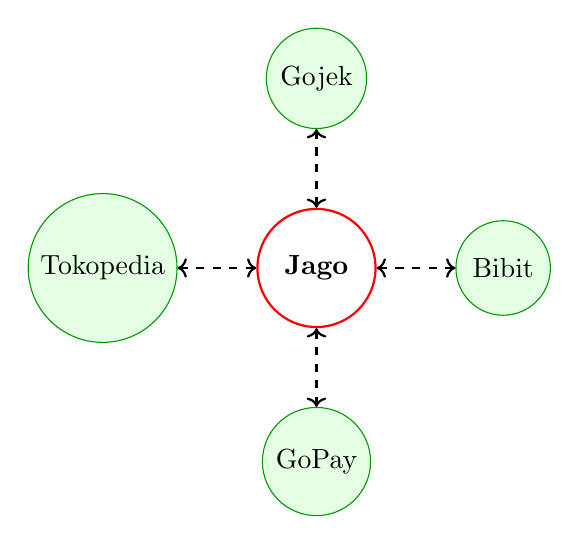
\begin{tikzpicture}
			\node (jago) [circle, draw=red, thick, fill=white, inner sep=2pt, minimum size=1.5cm] {\textbf{Jago}};

			\node (gojek) [circle, draw=green!60!black, fill=green!10, above=of jago, minimum size=1.2cm] {Gojek};
			\node (bibit) [circle, draw=green!60!black, fill=green!10, right=of jago, minimum size=1.2cm] {Bibit};
			\node (tokop) [circle, draw=green!60!black, fill=green!10, left=of jago, minimum size=1.2cm] {Tokopedia};
			\node (gopay) [circle, draw=green!60!black, fill=green!10, below=of jago, minimum size=1.2cm] {GoPay};

			\draw[<->, thick, dashed] (jago) -- (gojek);
			\draw[<->, thick, dashed] (jago) -- (bibit);
			\draw[<->, thick, dashed] (jago) -- (tokop);
			\draw[<->, thick, dashed] (jago) -- (gopay);
		\end{tikzpicture}
		\\ \footnotesize{Jago acts as the financial utility layer.}
	\end{columns}
\end{frame}

% --- Slide 6: Tech Transformation ---
\begin{frame}{Technological Transformation}
	Shift from Legacy Mainframe to Cloud-Native Architecture.

	\begin{columns}
		\column{0.5\textwidth}
		\textbf{Tech Stack Changes:}
		\begin{itemize}
			\item \textbf{Core:} Mambu (SaaS) on Google Cloud.
			\item \textbf{Architecture:} Microservices \& Open API.
		\end{itemize}
		\vspace{0.3cm}
		\textbf{Benefits:}
		\begin{itemize}
			\item \textbf{Scalability:} Auto-scale for events like 12.12.
			\item \textbf{Cost:} OpEx model (Pay-per-use).
			\item \textbf{Speed:} New products in weeks.
		\end{itemize}

		\column{0.5\textwidth}
		\centering
		% Using the user provided image
		\includegraphics[width=0.9\linewidth]{monolitic-vs-microservice.png}
		\vspace{0.2cm}
	\end{columns}
\end{frame}

% --- SLIDE 7: IT Impact Map ---
\begin{frame}{IT Impact Map Analysis}

	\centering
	% Make sure "it_impact_bank_jago.jpg" is in the folder
	\includegraphics[width=0.75\linewidth]{it_impact_bank_jago.jpg}

	\vspace{0.2cm}
\end{frame}

% --- SLIDE 8: Business Model Grid (Using User Image) ---
\begin{frame}{Business Model Evolution (Product-Market Grid)}

	\centering
	% Make sure "business_model_bank_Jago.jpg" is in the folder
	\includegraphics[width=0.75\linewidth]{business_model_bank_Jago.jpg}

	\vspace{0.2cm}
\end{frame}

\begin{frame}{Competitor: Bank Jenius}
	
	\centering
	% Make sure "it_impact_bank_jago.jpg" is in the folder
	\includegraphics[width=0.75\linewidth]{business_model_jenius.jpg}
	
	\vspace{0.2cm}
\end{frame}

\begin{frame}{Competitor: KakaoBank}
	
	\centering
	% Make sure "it_impact_bank_jago.jpg" is in the folder
	\includegraphics[width=0.75\linewidth]{business_model_kakao.jpg}
	
	\vspace{0.2cm}
\end{frame}

\begin{frame}{Strategic Comparison to Competitors}
	% Adjust font size to fit content comfortably
	\small 
	% Increase row height for readability
	\renewcommand{\arraystretch}{1.5} 
	
	\begin{tabularx}{\textwidth}{@{} l >{\raggedright\arraybackslash}X >{\raggedright\arraybackslash}X >{\raggedright\arraybackslash}X @{}}
		\toprule
		\textbf{Dimension} & \textbf{Bank Jago} & \textbf{Jenius} & \textbf{KakaoBank} \\ 
		\midrule
		\textbf{Origin} 
		& Legacy Transformation (Artos) 
		& Internal Spinoff (BTPN) 
		& Internet-Only License \\ 
		\textbf{Channel} 
		& Ecosystem (Gojek/Bibit) 
		& Standalone App 
		& Social (KakaoTalk) \\ 
		\textbf{Architecture} 
		& Cloud-Native (Mambu/GCP) 
		& Hybrid Digital Core 
		& Mobile-First Proprietary \\ 
		\textbf{Value Prop} 
		& Life-Centric (Invisible) 
		& Life-Finance Mgmt 
		& Social \& Convenient \\ 
		\textbf{Model} 
		& B2B2C (Partnership) 
		& B2C (Direct) 
		& B2C (Platform) \\ 
		\bottomrule
	\end{tabularx}
\end{frame}

% --- Slide 9: Financial Results ---
\begin{frame}{The Result: Financial Turnaround}
	\begin{columns}
		\column{0.5\textwidth}
		\textbf{Profitability:}
		\begin{itemize}
			\item \textbf{2019:} Net Loss IDR 165 Billion.
			\item \textbf{2021:} Net Profit IDR 86 Billion.
			\item \textbf{2023-24:} Sustained Profitability.
		\end{itemize}

		\vspace{0.3cm}
		\textbf{Scale:}
		\begin{itemize}
			\item Assets grew from IDR 733B to IDR 28.5T.
			\item User base grew to 15.3 Million.
		\end{itemize}

		\column{0.5\textwidth}
		\centering
		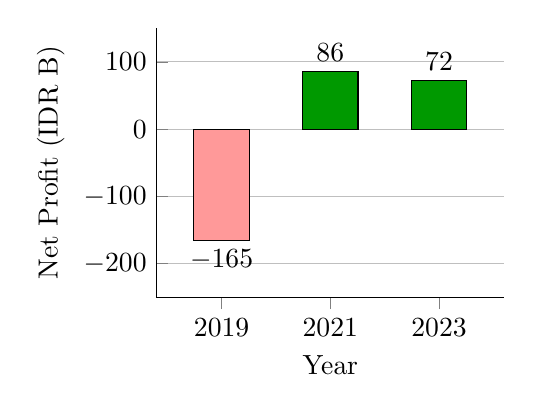
\begin{tikzpicture}
			\begin{axis}[
				ybar,
				symbolic x coords={2019, 2021, 2023},
				% --- FIX IS HERE ---
				xtick={2019, 2021, 2023}, % Explicitly force these 3 labels to appear
				% -------------------
				xlabel={Year},
				ylabel={Net Profit (IDR B)},
				ylabel near ticks,
				nodes near coords,
				nodes near coords align={vertical},
				enlarge x limits=0.3,
				ymin=-250, ymax=150,
				bar width=20pt,
				bar shift=0pt, % Keeps bars centered over the label
				width=6cm, height=5cm,
				axis lines*=left,
				ymajorgrids=true,
				]
				% Red bar (Loss)
				\addplot[fill=red!40] coordinates {(2019,-165)};
				% Green bars (Profit)
				\addplot[fill=green!60!black] coordinates {(2021,86) (2023,72)};
			\end{axis}
		\end{tikzpicture}
	\end{columns}
\end{frame}

% --- Slide 10: Conclusion ---
\begin{frame}{Conclusion}
	\begin{block}{Key Takeaways}
		\begin{enumerate}
			\item     \textbf{Strategy}: The pivot from a "Pipeline" model (Bank Artos) to a "Platform/Ecosystem" model (Bank Jago) unlocked exponential growth (from 50 thousand to 15 million customers) that was structurally impossible under the legacy model.

			\item \textbf{Capabilities}: The adoption of cloud-native infrastructure (Mambu/GCP) and agile organizational structures provided the speed and scalability required to execute the ecosystem strategy. This resolved the "organizational lag" that haunted Bank Artos.

			\item \textbf{Value}: The transformation corrected the fundamental insolvency of the legacy bank. By leveraging ecosystems to lower CAC and cloud tech to lower OpEx, Bank Jago converted a loss-making institution (BOPO 258\%) into a highly profitable and efficient digital bank (NPL 0.2\%).
		\end{enumerate}

	\end{block}

	\vspace{0.5cm}
	\centering
	\large{\textbf{"IT was not just a support tool; it was the driver of strategic renewal."}}
\end{frame}

% --- Slide 11: Q&A ---
\begin{frame}
	\centering
	\Huge \textbf{Thank You} \\
	\vspace{0.5cm}
	\Large Questions?
\end{frame}

\end{document}